\section{Method}
\label{sec:method}

\subsection{Airdrawing}
For hand tracking and gesture recognition, MediaPipe is an open source API that provides many real-time features. The team will use MediaPipe Hands, which uses "machine learning to track 21 3D landmarks [on the hand] from just a single frame" \cite{MP}. With these 21 3d landmarks, different gestures such as raising a specific finger can be detected. The airdrawing can then be programmed based on the user's hand landmarks shown in Figure~\ref{fig:mplm}. For example, if we want to detect whether index finger is raised, then we only need to check whether landmark 8 is higher than landmark 6 or 5. 

% [Talk about each gesture]

% paragraph in proposal. Will delete later
%The team will use OpenCV to capture each frame of the webcam. Each frame is passed into MediaPipe Hand to calculate the 21 3D landmarks of the hand. Based on the positions of these 21 3D landmarks, the program can detect the number of fingers that are raised. If right index finger is raised, then the program draws a point on the blank white canvas at the index finger's tip location. If all fingers minus the thumb are raised, then the image of the canvas is fed into our OCR model for \LaTeX\ conversion.

The team will follow similar approaches taken from Gulati et al's drawing application \cite{MPDrawing} for airdrawing. We used OpenCV to capture videos from the user's camera. Each frame of the video is then processed with MediaPipe Hands to track 21 3d landmarks. Given the relative location of each landmark, our code either draws more points on the white canvas, erase all drawings, or screenshot the current white canvas and feed it into the transformer to output the corresponding \LaTeX\ . Our airdrawing runs indefinitely until the user press the "Esc" key. 

\subsubsection{Airdrawing Modes} \label{sec:drawingmodes}
The airdrawing program has 3 modes: draw, clear, and feed. 

The user enables drawing mode if the only finger that the user raises is the right index finger. If 2 or 3 right fingers (can include right index finger) are raised up, then drawing would not happen. This way, the user can have the option to pause drawing and move his or her index finger to the next letter location. Then, the user could continue drawing by lifting only the index finger up.  

The implementation of the pixel drawing is inspired by this GeeksForGeeks post \cite{DrawMode}. Each time the drawing mode is activated, the position of the right index fingertip, which is MediaPipe Hand's landmark 8 in ~\ref{fig:mplm},  is stored in a deque. At the end of each frame processing, we used a for loop that draws a line between consecutive stored points. This allows the strokes to look continuous even though the index fingertip is sampled at each frame. Figure~\ref{fig:mpdraw} shows what drawing looks like.



The clear mode is activated when the user raises 4 left-hand fingers (no thumb). This will clear all strokes on the tracking image and the white canvas, as shown in Figure~\ref{fig:mpclear}. 

The feed mode saves the white canvas as a .bmp file and feed it into the transformer model for \LaTeX\ conversion, as shown in Figure~\ref{fig:mpfeed}.

\begin{figure}[h!]
    \centering
    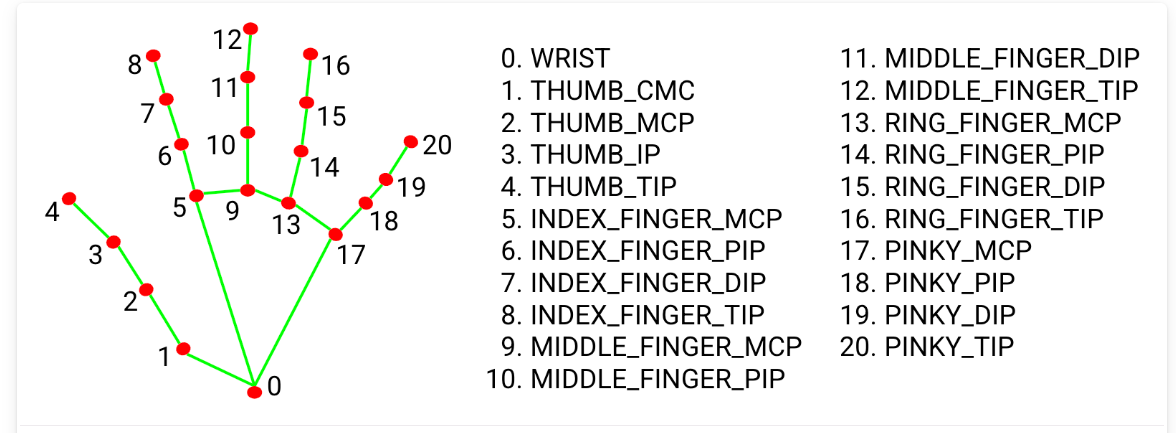
\includegraphics[width=8cm]{images/mplandmarks.png}
    \caption{MediaPipe Hand's 21 hand landmarks}
    \label{fig:mplm}
\end{figure}

\begin{figure}[h!]
    \centering
    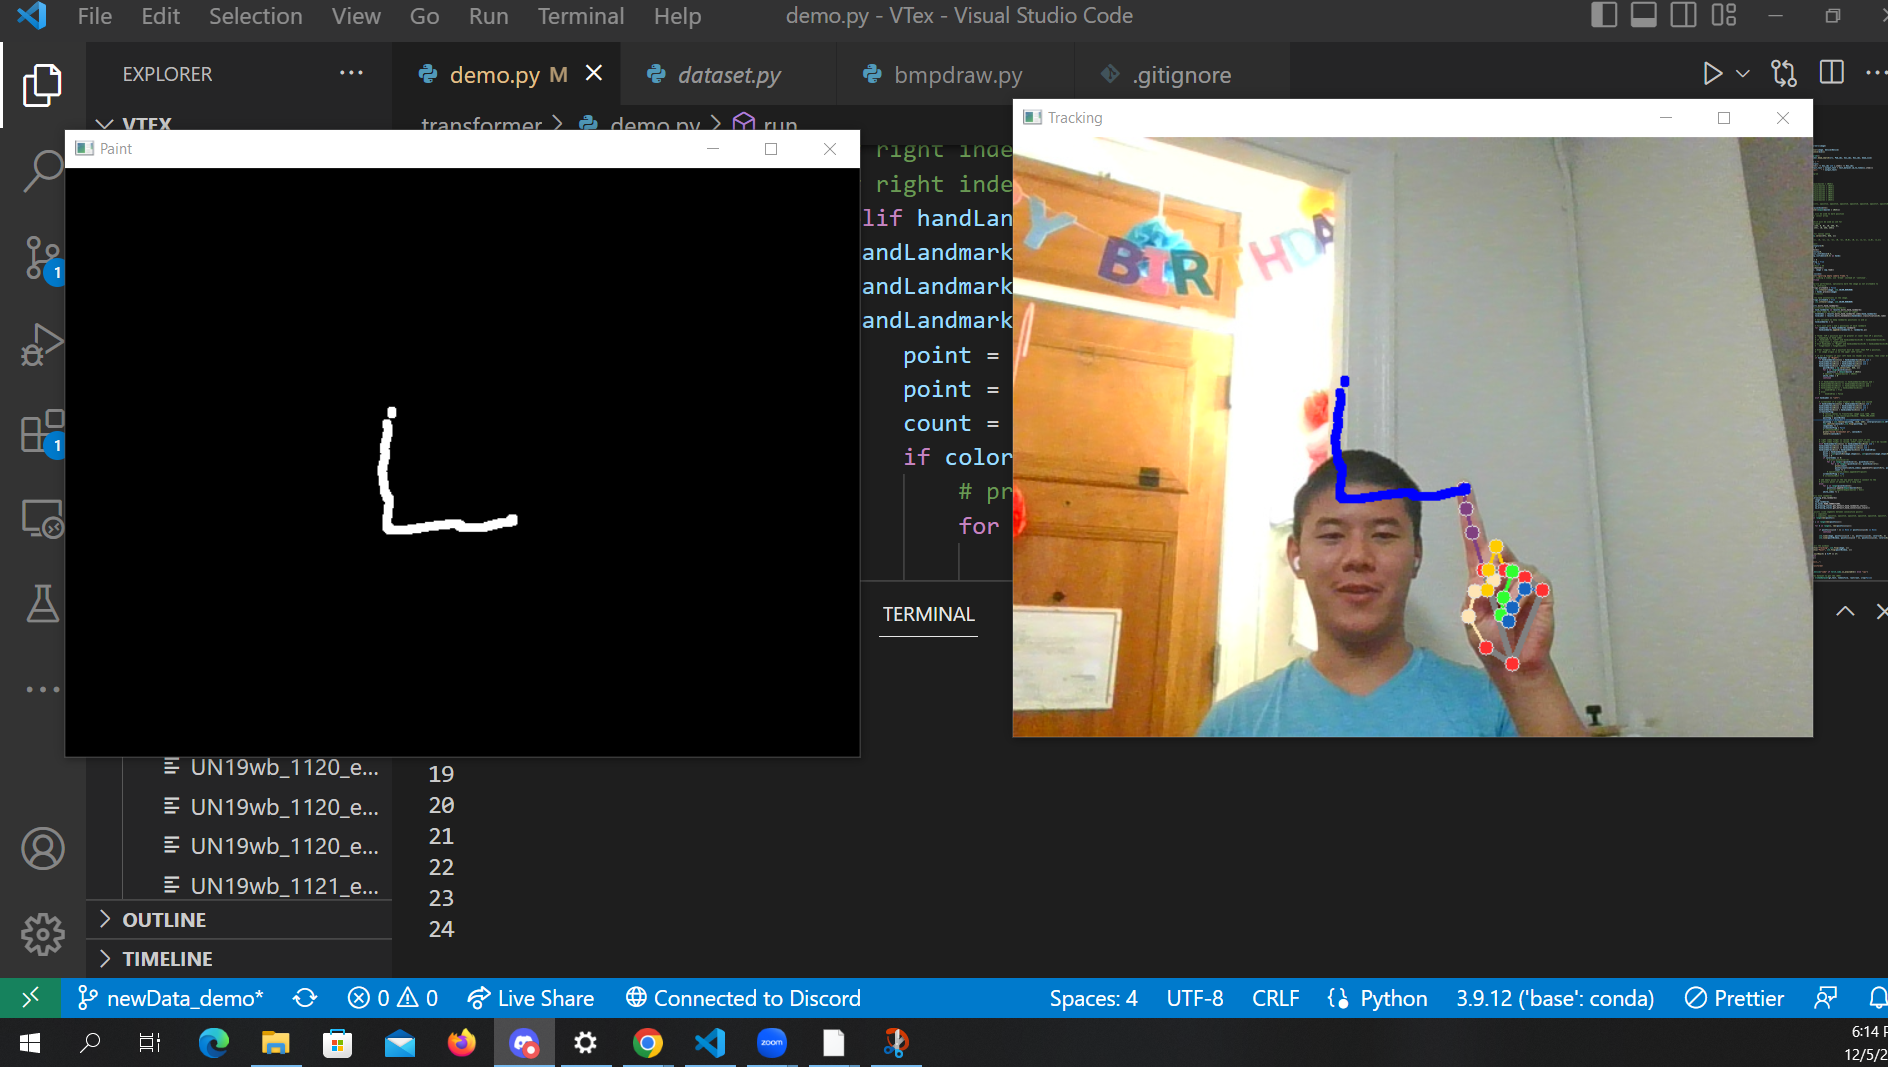
\includegraphics[width=8cm]{images/draw.png}
    \caption{When the right index finger is the only right finger raised, then the drawing will happen at its tip}
    \label{fig:mpdraw}
\end{figure}

\begin{figure}[h!]
    \centering
    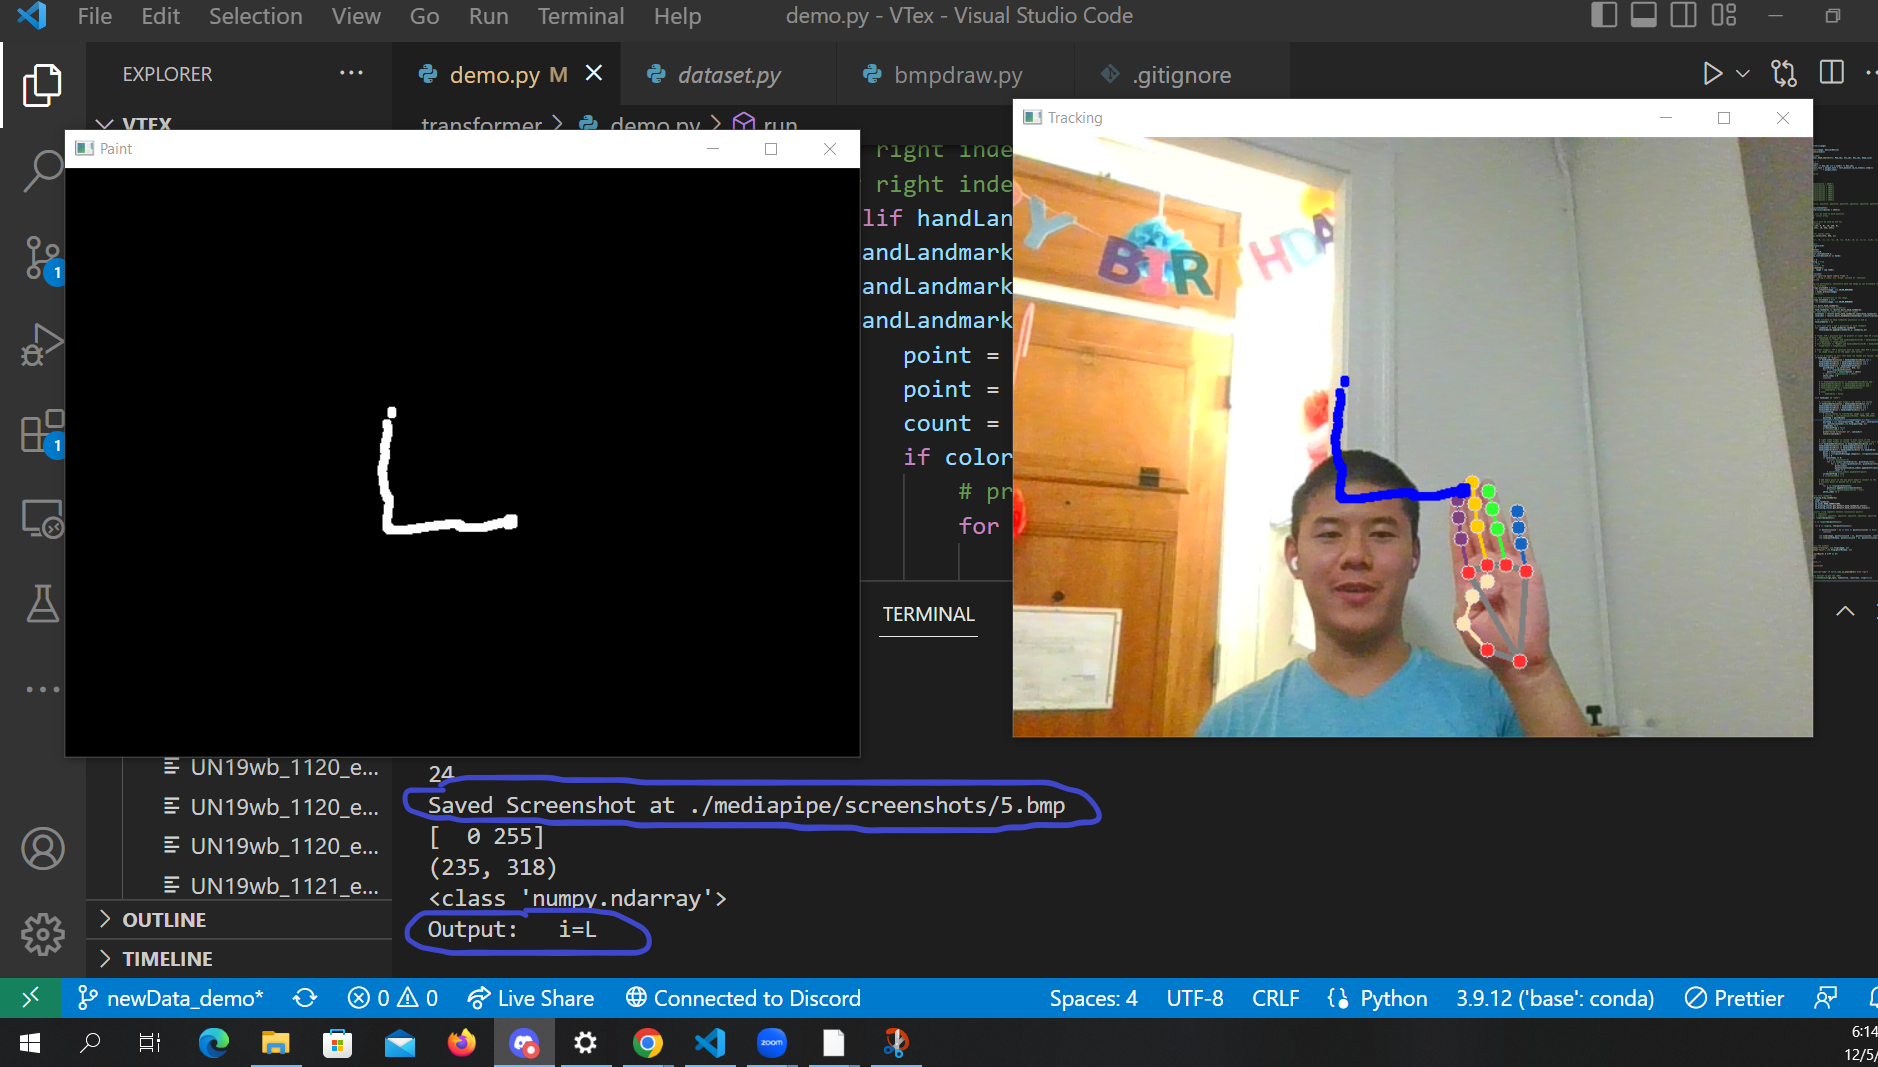
\includegraphics[width=8cm]{images/feed.png}
    \caption{When 4 right fingers are raised (no thumb), then the canvas will be saved as BMP image, and the program will pass the BMP image to the transformer for \LaTeX\ conversion. The program outputted \text{i=L}}
    \label{fig:mpfeed}
\end{figure}

\begin{figure}[h!]
    \centering
    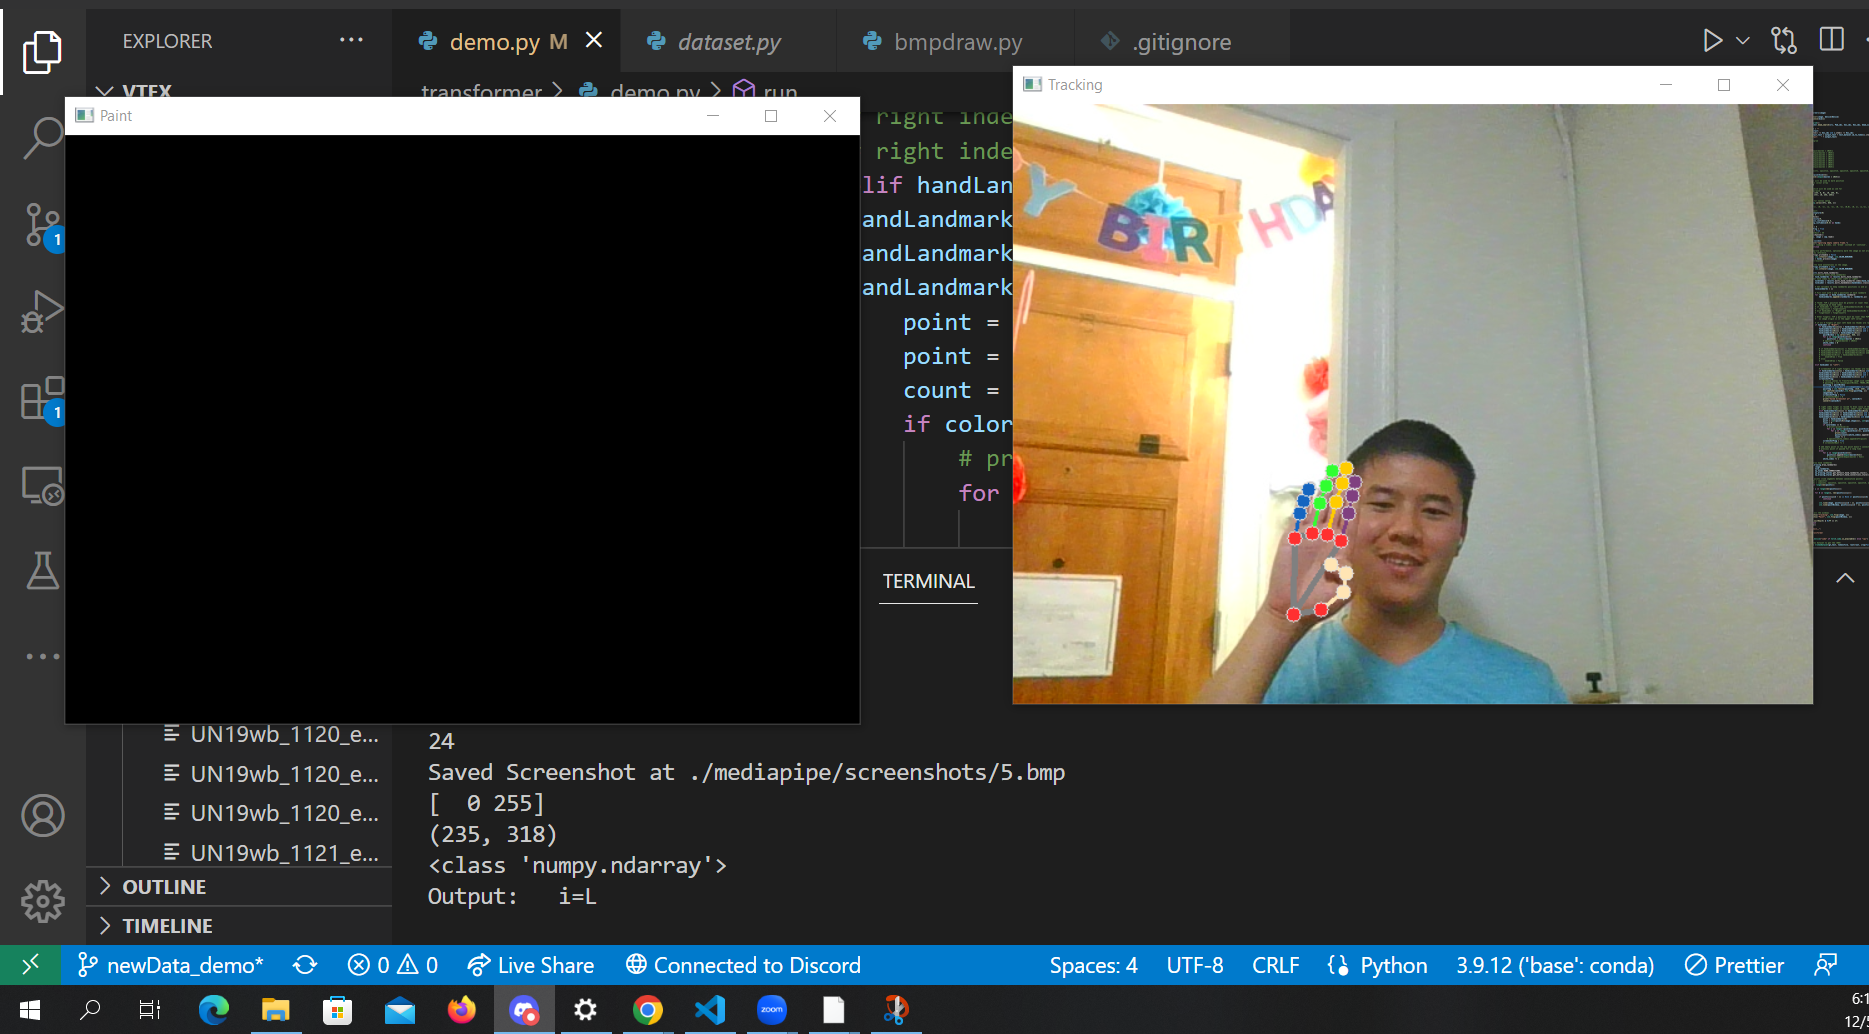
\includegraphics[width=8cm]{images/clear.png}
    \caption{When 4 left fingers are raised (no thumb), then the canvas will be cleared}
    \label{fig:mpclear}
\end{figure}
